\chapter{Configuration of user interfaces}
\label{chp:configurability}
\label{bkm:Configurability}This section looks at the various options available to user programs such as \PrBtr{} and \PrBtq{}.
In some cases, particularly with \PrBtr{} and \PrBtjchange{}, there is a perhaps bewildering array of options. It is not intended that
users should have to remember them all as they can be specified by default and overridden as required.

This is done by using \textit{configuration files} and environment variables. For example, the program \PrBtq{} may be configured to take
advantage of function keys and show a different set of information in a simplified format.

\begin{exparasmall}

Seq \ \ Job Name \ \ \ \ \ \ \ \ \ \ \ \ Args \ \ \ \ \ \ Date/Time
\ \ \ \ \ \ \ \ \ Prog

{}-{}-{}-{}-{}-{}-{}-{}-{}-{}-{}-{}-{}-{}-{}-{}-{}-{}-{}-{}-{}-{}-{}-{}-{}-{}-{}-{}-{}-{}-{}-{}-{}-{}-{}-{}-{}-{}-{}-{}-{}-{}-{}-{}-{}-{}-{}-{}-{}-{}-{}-{}-{}-{}-{}-{}-{}-{}-{}-{}-{}-{}-{}-{}-{}-{}-{}-

\ \ 1 \ \ start
\ \ \ \ \ \ \ \ \ \ \ \ \ \ \ \ \ \ \ \ \ \ \ \ \ \ 08/06/01 10:54
\ \ \ \ Canc

\ \ 2 \ \ Process directory \ \ \ /home \ \ \ \ \ 08/06/01 10:54

\ \ 3 \ \ Process directory \ \ \ /usr \ \ \ \ \ \ 08/06/01 10:54

\ \ 4 \ \ Process directory \ \ \ /tmp \ \ \ \ \ \ 08/06/01 10:54

\ \ 5 \ \ Collect data \ \ \ \ \ \ \ \ \ \ \ \ \ \ \ \ \ \ \ 08/06/01
10:54

\ \ 6 \ \ Error Handler \ \ \ \ \ \ \ \ \ \ \ \ \ \ \ \ \ \ 08/06/01
10:54

\ \ 7 \ \ cleanup
\ \ \ \ \ \ \ \ \ \ \ \ \ \ \ \ \ \ \ \ \ \ \ \ 08/06/01 10:54

\ \ 8 \ \ setup
\ \ \ \ \ \ \ \ \ \ \ \ \ \ \ \ \ \ \ \ \ \ \ \ \ \ 07/06/01 23:01
\ \ \ \ Done

\bigskip


{}-{}-{}-{}-F1-{}-{}-{}-{}-{}-F2-{}-{}-{}-{}-{}-F3-{}-{}-{}-{}-{}-F4-{}-{}-{}-{}-{}-F5-{}-{}-{}-{}-F6-{}-{}-{}-{}-{}-{}-{}-{}-{}-{}-{}-{}-{}-{}-{}-{}-{}-{}-{}-{}-{}-

\ \ \ help \ \ enable disable \ \ set \ \ \ view \ \ \ view

\ \ \ \ \ \ \ \ \ \ run \ \ \ run \ \ \ \ \ \ time \ \ job \ \ \ \ vars

{}-{}-{}-{}-{}-{}-{}-{}-{}-{}-{}-{}-{}-{}-{}-{}-{}-{}-{}-{}-{}-{}-{}-{}-{}-{}-{}-{}-{}-{}-{}-{}-{}-{}-{}-{}-{}-{}-{}-{}-{}-{}-{}-{}-{}-{}-{}-{}-{}-{}-{}-{}-{}-{}-{}-{}-{}-{}-{}-{}-{}-{}-{}-{}-{}-{}-{}-

\end{exparasmall}

This configuration could be specific to a particular user or activity.
In this case it is taken from a real configuration belonging to user
wally when using jobs in a queue named par. The screen display has been
changed as follows:

\begin{itemize}
\item The fields \exampletext{jobno}, \exampletext{Shell}, \exampletext{Pri}, \exampletext{Load} and \exampletext{Cond} have been removed.
\item The \exampletext{Time} field is changed from the abbreviated form to show time in full, \exampletext{Date/Time}. The \exampletext{Title}
field is widened to display more text.
\item The \exampletext{Argument} field has been added. This shows the differences between jobs which are identical except that they
use different data as specified in the arguments.
\item Column headings underlined and footer expanded to include function key reminders.
\end{itemize}
The set of jobs displayed has also been restricted to show just those in the queue named \exampletext{par} that belong to user
\exampletext{wally}.

This is what the standard configuration of \PrBtq{} looked like when invoked by user \exampletext{wally}, on
another terminal, at the same time:

\begin{exparasmall}

Seq Jobno \ \ User \ \ \ Title \ \ \ \ \ \ \ \ Shell \ \ Pri Load \ Time
\ Cond \ \ \ \ \ Prog

\ \ 0 340 \ \ \ \ wally \ \ e-mail:dial u sh \ \ \ \ \ 150 1000 \ 16:33

\ \ 1 734 \ \ \ \ tony \ \ \ prog\_a \ \ \ \ \ \ \ sh \ \ \ \ \ 150 1000
\ 06/02 \ \ \ \ \ \ \ \ \ \ Run

\ \ 2 1420 \ \ \ wally \ \ Output Exampl sh \ \ \ \ \ 150 1000 \ 29/01
\ \ \ \ \ \ \ \ \ \ Err

\ \ 3 735 \ \ \ \ tony \ \ \ prog\_b \ \ \ \ \ \ \ sh \ \ \ \ \ 150 1000
\ 08/02 A\_STATUS

\ \ 4 736 \ \ \ \ tony \ \ \ prog\_c \ \ \ \ \ \ \ sh \ \ \ \ \ 150 1000
\ 08/02 A\_STATUS

\ \ 5 439 \ \ \ \ wally \ \ wally \ \ \ \ \ \ \ \ sh \ \ \ \ \ 150 1000
\ \ \ \ \ \ \ \ \ \ \ \ \ \ \ \ \ Canc

\ \ 6 588 \ \ \ \ wally \ \ Also Sprach Z sh \ \ \ \ \ 150 1000 \ 04/02
\ \ \ \ \ \ \ \ \ \ Done

\ \ 7 564 \ \ \ \ wally \ \ Daily Update \ sh \ \ \ \ \ 150 1000
\ \ \ \ \ \ \ \ \ \ \ \ \ \ \ \ \ Run

\ \ 8 455 \ \ \ \ pior \ \ \ Simple Job \ \ \ sh \ \ \ \ \ 150 1000
\ 11/03 \ \ \ \ \ \ \ \ \ \ Abrt

\ \ 9 309 \ \ \ \ wally \ \ par:start \ \ \ \ sh \ \ \ \ \ 150 1000
\ 08/06 \ \ \ \ \ \ \ \ \ \ Canc

\ 10 310 \ \ \ \ wally \ \ par:Process d sh \ \ \ \ \ 150 1000 \ 08/06
**Cond**

\ 11 312 \ \ \ \ wally \ \ par:Process d sh \ \ \ \ \ 150 1000 \ 08/06
**Cond**

\ 12 313 \ \ \ \ wally \ \ par:Process d sh \ \ \ \ \ 150 1000 \ 08/06
**Cond**

\ 13 314 \ \ \ \ wally \ \ par:Collect d sh \ \ \ \ \ 150 1000 \ 08/06
**Cond**

\ 14 315 \ \ \ \ wally \ \ par:Error han sh \ \ \ \ \ 150 1000 \ 08/06
**Cond**

\ 15 316 \ \ \ \ wally \ \ par:cleanup \ \ sh \ \ \ \ \ 150 1000 \ 08/06
**Cond**

\ \ \ \ \ \ \ \ \ \ \ \ \ \ \ \ \ \ \ \ \ \ \ \ \ \ \ \ \ {}-{}- 9 more
jobs below -{}-

========================================================================

\end{exparasmall}

On the standard configuration jobs owned by users \exampletext{tony} and \exampletext{pior} can be seen along with other jobs
owned by \exampletext{wally} which were not relevant to the task in hand.

\section{Configuration files and environment variables}
Configuration files are called either \configurationfile{} in the current directory and only apply when
the command is run from that directory, or are located in a file \homeconfigpath{} off the user's home directory.
(Note that interpretation of \configurationfile{} in the user's home directory is still supported but this is deprecated as
the \configurationfile{} will be read twice when the current directory is the same as the home directory).

They are text files, containing environment variable type assignments. These ``environment variables''
may be used to specify program options and alternative message files.

Options to the user programs enable these files to be generated and edited automatically.

\subsection{Environment Variables}
The default options to each program may be overridden and others specified on the command line. A local default may be set up for each
program by putting the options in an environment variable.

For example using the \exampletext{{}-C} and the \exampletext{{}-r} options to \PrBtr{} to
submit a batch job in the \exampletext{Cancelled} state with a repeat time. If the job script is held in the file
\exampletext{fred} and the required repetition is every day, then the \PrBtr{} command will look something like
this:

\begin{expara}

\BtrName{} -r Days:1 -C fred

\end{expara}

If several batch jobs are being submitted, requiring the same options, it would be easier to put them into environment variable
\filename{\BtrVarname}. For example:

\begin{expara}

\BtrVarname={\textquotesingle}-r Days:1 -C{\textquotesingle}

export \BtrVarname{}

\end{expara}

These options would be automatically specified each time, until the environment variable is unset or changed. To override an environment
variable just re-specify the option on the command line. Command line options take precedence over environment variables. The general rule is
that for every option which ``does'' something, there is a corresponding option to ``undo'' it, to provide for this case.

When something more permanent is required \configurationfile{} or \homeconfigpath{} configuration files can be used.

\subsection{Configuration files}
A configuration file called \configurationfile{} may be put in the current directory to set options appropriate to running \ProductName{}
programs in this directory. The format of the file is similar to setting environment variables, but without the quotes or
``export'' statements.

For example:

\begin{expara}

\BtrVarname=-r Days:1 -C

\BtjlistVarname=-F {\textquotedbl}\%N \%H \%P{\textquotedbl}

\# ..... and so on

\end{expara}

The file may contain comment lines commencing with \exampletext{\#}. In fact any lines not understood are silently ignored.

As with environment variables the \configurationfile{} file may be overridden on the command line.

To specify default options for a user, whichever directory is in use, put a \homeconfigpath{} file off the user's
home directory. For example; to set \PrBtq{} to show only the user's jobs and variables on entry, put a \homeconfigpath{} file off the home directory containing the line:

\begin{expara}

\BtqVarname=-u \textit{user}

\end{expara}

This has a similar effect as setting up the environment variable \filename{\BtqVarname} in the user's \filename{.profile} or \filename{.login} file.

There is an order of precedence for options in home directory \homeconfigpath{} files, current directory \configurationfile{} files,
and in an environment variables. They are handled in the following order:

\begin{enumerate}
\item Any system-wide defaults are taken (e.g. the user's default job priority).
\item The home directory \homeconfigpath{} file is processed.
\item The home directory \configurationfile file{} is processed (for compatibility with previous versions).
\item The environment is processed.
\item The current directory \configurationfile{} file is processed.
\item Options on the command line are processed.
\end{enumerate}
Conflicting options encountered later completely override what came first, so that options specified on the command line will take priority
whatever else was encountered. As mentioned above, there is a ``reset'' type option for every ``set'' type option, so for example the
\PrBtr{} option \exampletext{{}-N} resets the option \exampletext{{}-C}.

The functions of the option letters can be re-assigned using alternative help message files. These may also be specified using environment
variables and/or the \configurationfile{} files.

\subsection{Environment variable or keyword names}
The table lists examples of the environment variables, or keywords in \configurationfile{} or \homeconfigpath{} files, used to hold various program
options. The environment variable or keyword for program options has the same name as the program it affects, except that it is in upper
case, for example the keyword for \PrBtq{} is \filename{\BtqVarname}, \PrBtr{} is \filename{\BtrVarname} etc.

The environment variable names are fixed, not taken from the program names. If any of the programs are given a different name the
environment variable names do not change.

To set the environment variable, the format is just the same as for the options in the corresponding command. For example using the Bourne or
Korn shells, type:

\begin{expara}

\BtrVarname={\textquotesingle}-C -r Minutes:30{\textquotesingle}

\BtqVarname={\textquotedbl}-u \$LOGNAME{\textquotedbl}

export \BtrVarname{} \BtqVarname{}

\end{expara}

The quotes (single or double) are required if spaces are included, which they usually are.

With the C shell type:

\begin{expara}

setenv \BtrVarname{} {\textquotesingle}-C -r Minutes:30{\textquotesingle}

setenv \BtqVarname{} {\textquotesingle}-u \$LOGNAME{\textquotesingle}

\end{expara}

There isn't any hard and fast rule about whether to use home \homeconfigpath{} or current directory \configurationfile{} files, or
environment variables.

In practice people tend to put ``comfort''-type options, such as help display options and the display of job numbers in the home directory.
Options specific to files in a given directory, such as batch job queue name and I/O redirections, would go in the current directory. Transient
requirements or those set up by applications invoking \ProductName{} programs are best put in the environment.

\section{User reconfiguration}
To allow maximum flexibility, all strings, such as screen headers, error and help messages, keystrokes and prompts used in \ProductName{} are taken
from a set of files. These message or help files can be edited and different versions of each file may be used for different contexts.
Some examples are:

\begin{enumerate}
\item Customising the interface on a system-wide basis by editing the default copies of the files.
\item Producing different versions to take advantage of the best facilities on different types of terminal.
\item Tailoring on an individual basis for each user by allowing each user to have access to their own version or versions of the files.
\item Tailoring for a group of users by making what seem to be their individual copies, read only symbolic links to a master copy.
\item Activity based versions pointed to by environment variables.
\end{enumerate}
As mentioned above all the keystrokes understood by \BtqName{} and \BtuserName{} are ``soft''. The functions may be redefined as
required. The following examples show the kinds of use these facilities can be put to:

\begin{enumerate}
\item Producing customised versions of the product incorporating site names, help messages etc. on the basic screen formats.
\item Providing ``seamless joins'' between \ProductName{} and other software with different function key sets.
\item Providing interfaces appropriate to different terminals, in particular, taking advantage of function keys provided on those
terminals.
\item Providing support for national languages - allowing different languages on different terminals on the same machine.
\end{enumerate}
\subsection{Message files}
The standard message files all live in the directory \helpdir{} (All of these names may be over-ridden by assignment to environment
variables as below). The files involved are:

\begin{center}
\begin{tabular}{l l}
\filename{btuser.help} & The configurable information for \PrBtuser{}\\
\filename{btq.help} & The configurable information for \PrBtq{}\\
\filename{filemon.help} & The configurable information for \PrBtfilemon{} and \PrXmfilemon{}\\
\filename{xmbtq.help} & Message file for \PrXmbtq{}\\
\filename{xmbtr.help} & Message file for \PrXmbtr{}\\
\filename{xmbtuser.help} & Message file for \PrXmbtuser{}.\\
\filename{btrest.help} & Which contains all the configurable information for remaining user programs\\
\filename{btint-config} & containing the configurable information for the programs internal to \ProductName{}\\
\end{tabular}
\end{center}
The files are found by default from \progsdir{} as specified.

To specify an alternative file, use the configuration file or environment variable mechanism previously described. The following
table lists the environment variables and/or keywords used for various
user programs:

\begin{center}
\begin{tabular}{|l l|}
\hline
\bfseries Environment variable or keyword & \bfseries Description\\\hline
\filename{BTQCONF} & \PrBtq{} message file\\
\filename{BTUSERCONF} & \PrBtuser{} message file\\
\filename{FILEMONCONF} & \PrBtfilemon{} and \PrXmfilemon{} message file\\
\filename{XMBTQCONF} & \PrXmbtq{} message file\\
\filename{XMBTRCONF} & \PrXmbtr{} message file\\
\filename{XMBTUSERCONF} & \PrXmbtuser{} message file\\
\filename{BTRESTCONF} & Message file for other utilities\\\hline
\end{tabular}
\end{center}
For example to use an alternative message file for \PrBtq{}, specify its use by means of the environment
variable setting:

\begin{expara}

BTQCONF={\textasciigrave}pwd{\textasciigrave}/my-\BtqName-file\newline
export BTQCONF

\end{expara}

It is important to specify the full path name, otherwise the file will be searched for in whatever directory is current.

Just like the command line options, the message file may be specified in a configuration file \homeconfigpath{}
file in the home directory or \configurationfile{} file in the current directory. If it is located in the home directory,
it will apply whichever directory is current, otherwise it will apply to the current directory.

The format of lines in the \configurationfile{} files is similar to that used to set environment variables in the shell. For example:

\begin{expara}

BTQCONF=\$HOME/lib/mybtq.help\$TERM

\end{expara}

Note that environment variable names are also expanded here, so in this example the user is intending to specify a different file according to
the setting of the \filename{TERM} environment variable.

There are 3 facilities in the expansion of these lines intended to assist the user to supply defaults etc:

Firstly, as with the shell, sequences of the form \exampletext{\$\{VAR-default\}} are replaced by the value of
environment variable \exampletext{VAR} if it exists, and otherwise the default string specified.

Secondly the sequence \filename{\$0} is replaced by the name (or the last component of the file name) by which the program was
invoked. For example

\begin{expara}

BTRESTCONF=\$HOME/lib/helps/\$0.help

\end{expara}

relates the message file's name to the name of the program invoked. Hence it would be \filename{\BtjlistName.help} if
\PrBtjlist{} was run, \filename{\BtvarName.help} for \PrBtvar{}, and so on.

Finally, if it cannot find the file specified, then an attempt will be made to find a file name constructed by deleting the last part of the
file name from the path and substituting the standard name (\filename{\BtqName.help}, \filename{btrest.help} etc),
before giving up.

For example in the above case, if the files \filename{\BtjlistName.help} or \filename{\BtvarName.help}
could not be found in the directory \exampletext{\$HOME/lib/helps}, then a further try would be
made with the standard name \filename{btrest.help} to give the file name \exampletext{\$HOME/lib/helps/btrest.help}.

As for the argument keywords and environment variables, the current directory \configurationfile{} file takes precedence over
environment variables, if any, which in turn take precedence over the home directory \homeconfigpath{} file. However once the
keyword is found in one of those places, the remainder are not searched; this means that if a non-existent file is specified, say in
the current directory \configurationfile file{}, then the program will abort without looking in the other places.

\subsection{File format}
It is easiest to work on these files by copying one of the supplied ones and starting from there. The files are plain text which can be edited
with any suitable text editor.

Message files have a common format and notation:

\begin{itemize}
\item Blank lines are ignored.
\item Comment lines, beginning with \exampletext{\#}, are ignored.
\item All other lines are \textit{definitions}.
\end{itemize}
Example lines within the files might be:

\begin{expara}

K400:?\newline
1K500:o,*\newline
100P:Ok to delete (Y/N)\newline
E100:Unknown command - expecting job queue control\newline
H400:Please reply Y or N

\end{expara}

The general form of the definition lines is:

\begin{enumerate}
\item An optional \textit{state code}, denoting the state of the program in which the line applies.
\item A key letter, denoting the function, i.e. key definition, prompt, error or help message etc.
\item A code number for which the program looks when it requires a particular line.
\item A colon preceding the definition of the item.
\end{enumerate}
The state and code numbers are arbitrary and compiled into the relevant programs.
Hopefully the context and the comments in the supplied files will make the situations in which they are used clear enough.

The types of entries given by the key letters are as follows:

\begin{center}
\begin{tabular}{l l}
\exampletext{K} & a key mapping\\
\exampletext{H} & a ``\textit{help}'' or similar type message\\
\exampletext{E} & an \textit{error} or other information message\\
\exampletext{P} & a ``\textit{prompt}'' or other screen field\\
\exampletext{N} & a numeric parameter\\
\exampletext{A} & an \textit{option} definition or an \textit{alternative}\\
\exampletext{AD} & a default \textit{alternative}\\
\end{tabular}
\end{center}
In addition there are screen heading lines, which have a slightly different format using other letters, defined later.

\subsubsection{Key definitions}
Key definitions are read in when the program is first started. As a result conflicts, where a key is defined for two or more different
uses, and other errors are detected before further processing is done.

There are two types of key definition; \textit{global} definitions which apply everywhere within the program, and \textit{local} definitions,
which only apply in a particular context, enabling you to use the same key in another context for a different purpose.

A global key definition looks like this:

\begin{expara}

K400:?

\end{expara}

whilst a local definition looks like this:

\begin{expara}

1K500:o

\end{expara}

The first number is referred to as a \textit{state code}. The number after the \exampletext{K} gives the internal code into which
the key sequence is translated and used to select the program action.

In all the contexts where state codes apply, there is a help message supplied with the same code as the state code. For example state 1
corresponds to the state where the cursor is in the job queue, keys relevant to this state only are prefixed with this state code, and the
help message lines for this state start with ``\exampletext{H1:}''.

The balance of the key definition gives the character sequences which make up the key definition; these will be translated to the internal
code. In the above examples the character \exampletext{?} is globally translated to the internal code 400 and
\exampletext{o} to 500 in state 1.

Non-printing and control characters are represented using the prefixes \exampletext{{\textbackslash}} and
\exampletext{\^{}}. In particular commas must be represented as \exampletext{{\textbackslash},} and spaces and tabs as
\exampletext{{\textbackslash}s} and \exampletext{{\textbackslash}t} respectively.

To give two or more keys for a given command, separate them by commas, as follows:

\begin{expara}

K400:?,*

\end{expara}

Hence the need to represent commas using \exampletext{{\textbackslash},} as just mentioned. The symbols
for the non-printing characters are:

\begin{center}
\begin{tabular}{|l l|}\hline
\bfseries Character & \bfseries Description\\\hline
\exampletext{\^{}a} etc & Appropriate control character\\
\exampletext{\^{}\^{}} & Denotes a single \exampletext{\textit{\^{}}}\\
\exampletext{{\textbackslash}{\textbackslash}} & Denotes a single \exampletext{\textit{{\textbackslash}}}\\
\exampletext{{\textbackslash},} & Denotes a \exampletext{\textit{,}}\\
\exampletext{{\textbackslash}s} & Space\\
\exampletext{{\textbackslash}t} & Tab\\
\exampletext{{\textbackslash}b} & Backspace\\
\exampletext{{\textbackslash}e} & Escape\\
\exampletext{{\textbackslash}n} & Linefeed\\
\exampletext{{\textbackslash}r} & Carriage return\\
\exampletext{{\textbackslash}f} & Form feed\\
\exampletext{{\textbackslash}xnn} & Character given by hexadecimal \textit{nn}\\
\exampletext{{\textbackslash}}\exampletext{\textit{nnn}} & Character given by octal \textit{nnn}\\
\exampletext{{\textbackslash}kkeyname} & String or character given by the \textit{keyname} (see below)\\\hline
\end{tabular}
\end{center}
Many keys, in particular cursor and function keys, generate multi-character sequences. The sequences can be just written out thus:

\begin{expara}

K406:{\textbackslash}e[A

\end{expara}

The whole of the sequence up to the end or to a comma will be searched for and translated to the given internal code when it occurs. The
arrival of the characters will be timed so it should be possible to distinguish between key sequences with similar prefixes (often the case
with cursor and function keys) and the effect of typing the component characters separately. This particularly affects the escape character,
which on its own is commonly used to abort input, but which also invariably prefixes function and cursor key sequences.

If necessary the timing of the arrival of characters can be tuned by means of the environment variable \filename{KEYDELAY}. This is
set to the number of 1/10ths of a second to wait between the characters of a suspected function key.

If another character is not received within this time, the character will be assumed to be a single key, otherwise it is taken as the start
of a function key. The default for \filename{KEYDELAY} is 3/10ths of a second, which should work correctly for the vast majority
of terminals.

If this value is too low, then function keys may not always be recognised, whilst if it is too high, then the response to a single
escape character, when required, will appear to be slow.

\paragraph{Special key sequences.}
As well as the control and non-printing characters which may be inserted using the sequences
``\filename{{\textbackslash}n}'' and ``\filename{\^{}c}'' etc, additional constructs introduced by
``\filename{{\textbackslash}k}'' are provided to import the user's choice of keys for erase, kill etc,
and the \textit{termcap} or \textit{terminfo} definitions of some of the special function keys on the terminal.

There are two problems which can arise:

\begin{enumerate}
\item Choices of single-character keys often conflict with existing uses of the same key, but not in a consistent way for each user or terminal.
For example:

\begin{enumerate}
\item The character \textit{ctrl}{}-U (\^{}U) is defined in the supplied files as ``scroll-half up''. Many people use
this as a kill character.
\item Some terminals have cursor keys which generate a single character. For example the left cursor key may generate a backspace
(\textit{ctrl}{}-H) character which cannot be distinguished from a real backspace character (or indeed \textit{ctrl} and `h').
\end{enumerate}
\item \textit{termcap} and \textit{terminfo} files may contain incorrect specifications about what sequences are generated by cursor and
function keys. This may not always be the fault of the files themselves if the user has extensively used softkey-setup facilities on the
terminal.
\end{enumerate}
The way to import these values is to use the sequence ``{\textbackslash}k'' followed by the symbolic name of the required item. The items available are:

\begin{center}
\begin{tabular}{|l l|}\hline
\bfseries Symbolic Name & \bfseries Meaning\\\hline
\exampletext{{\textbackslash}kINTR} & user's interrupt key\\
\exampletext{{\textbackslash}kKILL} & user's kill key\\
\exampletext{{\textbackslash}kERASE} & user's erase key\\
\exampletext{{\textbackslash}kQUIT} & user's quit key\\\hline
\end{tabular}
\end{center}
which are looked up on entry to \PrBtuser{} or \PrBtq{} from the \textit{termio} or \textit{stty}
settings, as set by \progname{stty}, and:

\begin{center}
\begin{tabular}{|l l|}\hline
\bfseries Symbolic Name & \bfseries Meaning\\\hline
\exampletext{{\textbackslash}kUP} & string sent by up arrow key\\
\exampletext{{\textbackslash}kDOWN} & string sent by down arrow key\\
\exampletext{{\textbackslash}kLEFT} & string sent by left arrow key\\
\exampletext{{\textbackslash}kRIGHT} & string sent by right arrow key\\
\exampletext{{\textbackslash}kHOME} & string sent by home key\\
\exampletext{{\textbackslash}kFnn} & string sent by function key F\textit{nn}\\\hline
\end{tabular}
\end{center}
which are looked up in the \textit{terminfo} or \textit{termcap} database for the terminal type specified in the environment variable
\filename{TERM}.

To use these sequences, put the relevant one in place in the key definition for example:

\begin{expara}

K400:?,{\textbackslash}kF1

K406:k,{\textbackslash}kUP

\end{expara}

If something does go wrong due to one of the two problems given above, the program will display some error messages and terminate. For example

\begin{expara}

State 5 setup error - clash on character 08 with previously-given value

420 and new value 530

\end{expara}

In this case the problem can be pinpointed by looking for a key definition with 420 in (this is the code for erase last character) and
another with 530 in (left cursor in some fields). This particular message often appears on terminals where left cursor is the same as
backspace. In other words \exampletext{{\textbackslash}kLEFT} and \exampletext{{\textbackslash}kERASE} produce the same
result - control-H or hexadecimal 08.

The other thing which might happen is that the function keys do not work properly or the message \exampletext{Undefined key sequence}
is displayed. This is because there is an incorrect \textit{termcap} or \textit{terminfo} file, or function keys have been reset.

A common problem on VT100-based terminals is that there are four settings depending upon which combination is selected of
``normal'' or ``application'' cursor keys and ``numeric'' or ``application'' keypad. It is possible that
the \textit{terminfo} file will assume one of the combinations whilst the terminal will be set to one of the other three.

This particularly affects cursor keys which are often defined in the \textit{terminfo} file to be
\exampletext{{\textbackslash}eOA}, \exampletext{{\textbackslash}eOB}, \exampletext{{\textbackslash}eOC} and
\exampletext{{\textbackslash}eOD} (application keys) for up, down, right and left cursor respectively whilst the terminal when
switched on generates the ``normal'' cursor keys \exampletext{{\textbackslash}e[A}, \exampletext{{\textbackslash}e[B},
\exampletext{{\textbackslash}e[C} and \exampletext{{\textbackslash}e[D} respectively.
If this problem occurs we suggest spelling out the combinations explicitly, for example

\begin{expara}

K406:k,{\textbackslash}e[A,{\textbackslash}eOA

K407:j,{\textbackslash}e[B,{\textbackslash}eOB

\end{expara}

Remember to adjust any help and error messages to reflect the keys that have been changed.

\paragraph{Help and error messages}
Help and error messages are treated almost identically. The only real difference is that they are displayed slightly differently.

The text to be displayed is given on as many lines as required with the same prefix, for example:

\begin{expara}

E1:Unknown command - expecting job queue control

E100:Type ? for help

H1:? - help (this file)

H1:\^{}L - redraw screen

\end{expara}

There are specific variables or strings which it is helpful for the help or error message to quote in the message. They are inserted using
``parameters'' introduced by \exampletext{\%} as follows:

\begin{center}
\begin{tabular}{|l l|}
\hline
\bfseries Parameter & \bfseries Meaning\\\hline
\exampletext{\%c0} to \exampletext{\%c9} & Numeric parameter 0 to 9 interpreted as a character, or hexadecimal if non-printing\\
\exampletext{\%d0} to \exampletext{\%d9} & Numeric parameter 0 to 9 interpreted in decimal\\
\exampletext{\%E} & System error message\\
\exampletext{\%F} & Name of message file\\
\exampletext{\%f} & Floating-point number (2 decimal places)\\
\exampletext{\%G} & Group name of \textit{effective gid}\\
\exampletext{\%g0} to \exampletext{\%g9} & Numeric parameter 0 to 9 interpreted as group id.\\
\exampletext{\%H} & Group name of \textit{real gid}\\
\exampletext{\%N} & Host name\\
\exampletext{\%P} & Program name\\
\exampletext{\%p} & Numeric process id\\
\exampletext{\%R} & User name of \textit{real uid}\\
\exampletext{\%s} & Primary string parameter\\
\exampletext{\%t} & Secondary string parameter\\
\exampletext{\%U} & User name of \textit{effective uid}\\
\exampletext{\%u0} to \exampletext{\%u9} & Numeric parameter 0 to 9 interpreted as user id\\
\exampletext{\%x0} to \exampletext{\%x9} & Numeric parameter 0 to 9 interpreted in hexadecimal\\\hline
\end{tabular}
\end{center}
The actual parameters are provided by the context. Some of the information (program name, process ID, error code, real and effective
user \& group IDs) is always available. The rest of the information (the 2 string arguments, the 10 parameters) is set up as required for
each error message by the calling program. The only way to discover what has been passed is to examine the error message, as given in the
standard help/message files, and to use the same parameters, possibly with a different format.

\paragraph{Option syntax}
There are two alternatives to using the standard single letter command-line options:

\begin{enumerate}
\item You can invoke options with keywords such as \exampletext{+priority} or \exampletext{{}-{}-priority} instead of or as well as
single-letter options such as \exampletext{{}-p}.
\item Alternative option letters and keywords may be specified by use of different message files.
\end{enumerate}
Option syntax is defined by means of lines of the form

\begin{expara}

A119:p,priority

\end{expara}

As with other parts of the file, there is an internal state code, in this case 119, to denote the action to take. Alternatives are specified
after the colon and separated by commas. They may consist of either:

\begin{enumerate}
\item Any single printing character, as for p in the above example, which denotes a ``\exampletext{{}-}'' type argument,
thus \exampletext{{}-p}. The character is taken exactly as given, and can be any printing character
(a comma or \exampletext{{\textbackslash}} must be escaped using a \exampletext{{\textbackslash}} thus \exampletext{{\textbackslash},}
\exampletext{{\textbackslash}{\textbackslash}} but these, especially the latter, are very strongly discouraged, for obvious reasons).
\item A keyword consisting of alphanumeric characters, \exampletext{{}-} and \exampletext{\_} starting with a letter, denoting a keyword-type argument, thus
\exampletext{+priority} or \exampletext{{}-{}-priority}. Letters in the keyword are case insensitive.
\end{enumerate}
It is not compulsory to define either single-character or keyword type options for any function. If one type is left out then only the other
type will be available. If both types are left out the option will not be available.

If you leave out option syntax definitions out of the file altogether, then a default set of options consisting only of the single-character
variants of the options as defined in this manual for each program will be supplied.

Please be careful before getting carried away!

When a job is unqueued from \PrBtq{}, the program \progname{jobdump} will be run and will pick up the version of the message files as for \PrBtr{}. It starts with configuration files in the current directory from which \PrBtq{} was invoked, using the options specified to
generate arguments for a \PrBtr{} command. The same considerations apply to options saved using
\exampletext{+freeze-current} and \exampletext{+freeze-home} options to various commands.

Take care because this means that with completely different option definitions in various places, the current set may be inappropriate
(particularly with the unqueue operation). It is best not to have different specifications for the options in different places on the
machine(s). For example do not set things up so that \exampletext{\BtrName{} -C} means submit job cancelled in some
contexts but something different elsewhere.

\paragraph{Alternatives}
In many contexts, such as the progress code of a job, it is necessary to select a string according to a numeric value. These strings are
presented together in the form:

\begin{expara}

{\textless}state code{\textgreater}A{\textless}numeric
parameter{\textgreater}:{\textless}text{\textgreater}

\end{expara}

For example (from \filename{btq.help})

\begin{expara}

100AD0:\newline
100A1:Done\newline
100A2:Err\newline
100A3:Abrt\newline
100A4:Canc\newline
100A5:Init\newline
100A6:Strt\newline
100A7:Run\newline
100A8:Fin

\end{expara}

The numeric parameters 0 to 8 represent the numeric values of the progress codes and the alternatives for internal state 100 yield the
appropriate string.

These alternatives are also used in questions requiring a choice; a prompt will be generated consisting of all the alternatives in the
order given. The default alternative is given by \exampletext{D}.

Comments in the supplied message files show where this applies.

\paragraph{Prompts}
Strings introduced with sequences such as 100P: are \textit{prompts}. These are transient messages which are generated in various places such
as:

\begin{itemize}
\item Messages at the bottom of the screen indicating so many jobs below.
\item Prompts for user input, e.g. when a job or variable parameter is being changed
\item Prompts for confirmation on ``sensitive'' commands, like deleting a job.
\end{itemize}
Some prompts have parameters in (such as the ``\exampletext{n jobs below}'' message), which are introduced with a \exampletext{\%}
sequence such as \exampletext{\%s} or \exampletext{\%d}. These are similar to the constructs in the C programming language \progname{printf}
function\footnote{Exactly similar in fact, as it uses the \progname{printf} function.}.

\paragraph{Numeric parameters}
There are some sequences of the form

\begin{expara}

1000N1001

\end{expara}

in the files. These are used in 4 places:

\begin{enumerate}
\item In the \PrBtq{} ``job options'' screen, to configure the order of prompts and the prompt to start with.
\item In the \PrBtuser{} display or set privileges options, to configure the order to present the privileges.
\item In the ``save options'' screens in both \PrBtq{} and \PrBtuser{} to configure the order in which the prompts are presented.
\item To present certain numeric parameters, such as the default number of repeat units, or default constant for increment/decrement of
variables.
\end{enumerate}
Please see the comments in the supplied files for how to adjust these parameters.

\paragraph{Titles}
The screen titles used by \PrBtq{} and \PrBtuser{} are handled slightly differently.
Although they can be multi-line, each line of the title is taken from a different message number. For example,
\exampletext{J}\exampletext{\textit{n}}\exampletext{:}
is the format for the \textit{n}th line of the title for the \PrBtq{} jobs list. (The \exampletext{J}
stands for ``jobs''). The default is:

\begin{expara}

J1:j

\end{expara}

This creates a one line title which has names of each column generated
automatically.

If the automatically generated title is not suitable it may be replaced by removing the letter \exampletext{j} and putting the desired
text after the : like this

\begin{expara}

J1:Seq Jobnum Owner Description ... \textit{and so on}

\end{expara}

The footer for the jobs screen is specified by lines starting \exampletext{Fn:} for example

\begin{expara}

F1:========================================= ...\newline
F2:Batch Queue \%P Acme Ltd ...

\end{expara}

Similarly the title and footer for the \PrBtq{} variable list is taken from lines starting with
\exampletext{Vn:} and \exampletext{Gn:} respectively. Each variable is described over two lines, hence two automatically
generated column headings are available. The default title for the variable list uses these auto-generated headings like is:

\begin{expara}

V1:1\newline
V2:2\newline
V3:-{}-{}-{}-{}-{}-{}-{}-{}-{}-{}-{}-{}-{}-{}-{}-{}-{}-{}-{}-{}-{}-{}-{}-{}-{}-{}-{}-{}-{}-{}-{}-{}-{}-{}-{}-{}-{}-{}-{}-{}-{}-{}-{}-{}-

\end{expara}

The height of the title or footer is given by the highest-numbered line specified - 3 in the above case. If line \exampletext{V2:} had
not been specified a blank line would be inserted between lines \exampletext{V1} and \exampletext{V3}.

Program \PrBtuser{}, when invoked for interactive operation by the \exampletext{\BtuserName{} -i} command, takes the
title and footer specifications from lines starting \exampletext{Ln:} and \exampletext{Fn:} respectively.

It is permissible to omit any or all of these titles completely if desired, leaving more space on the screen for jobs, variables or users,
as the case may be.

\paragraph{Enhancements and line drawing in headers}
It is possible to specify screen enhancements and line drawing characters within headers. To do this, the following sequences are
interpreted within headers lines.

\begin{center}
\begin{tabular}{l l}
\exampletext{{\textbackslash}B} & Set bold mode\\
\exampletext{{\textbackslash}D} & Set dim mode\\
\exampletext{{\textbackslash}F} & Set flashing mode\\
\exampletext{{\textbackslash}U} & Set underlined mode\\
\exampletext{{\textbackslash}I} & Set inverse video mode\\
\exampletext{{\textbackslash}S} & Set standout mode\\
\exampletext{{\textbackslash}N} & Reset to normal mode\\
\end{tabular}
\end{center}
The effect of the these sequences are cumulative and apply until the end of the line or until the \exampletext{{\textbackslash}N}
sequence is encountered.

For example the line

\begin{expara}

{\textbackslash}UExample{\textbackslash}N Header

\end{expara}

would be displayed as

\begin{expara}

\underline{Example Header}

\end{expara}

Note that, not all \textit{terminfo} files define all of the various enhancements, also that ``standout'' mode is
usually some arbitrary combination of the others.

The line-drawing set, if available, is separately invoked by use of sequences thus;

\begin{tabular}{l p{13cm}}
\exampletext{{\textbackslash}L} & Turn on line drawing mode and display upper left corner line drawing symbol.\\
\exampletext{{\textbackslash}l} & Turn on line drawing mode and display lower left corner line drawing symbol.\\
\exampletext{{\textbackslash}R} & Turn on line drawing mode and display upper right corner line drawing symbol.\\
\exampletext{{\textbackslash}r} & Turn on line drawing mode and display lower right corner line drawing symbol.\\
\exampletext{{\textbackslash}{\textbar}} & Turn on line drawing mode and display vertical edge line drawing symbol.\\
\exampletext{{\textbackslash}-} & Turn on line drawing mode and display horizontal edge line drawing symbol.\\
\exampletext{{\textbackslash}+} & Turn on line drawing mode and display internal intersection line drawing symbol.\\
\exampletext{{\textbackslash}{\textless}} & Turn on line drawing mode and display intersection of horizontal line and
left edge `T' line drawing symbol.\\
\exampletext{{\textbackslash}{\textgreater}} & Turn on line drawing mode and display intersection of horizontal line
and right edge `T' line drawing symbol.\\
\exampletext{{\textbackslash}\^{}} & Turn on line drawing mode and display intersection of vertical line and top edge `T' line drawing symbol.\\
\exampletext{{\textbackslash}V} & Turn on line drawing mode and display intersection of vertical line and bottom edge `T' line drawing symbol.\\
\end{tabular}

Once line-drawing mode is set, then any of the above characters which immediately follow are interpreted without needing to have a
``\exampletext{{\textbackslash}}''in front, so for example

\begin{expara}

{\textbackslash}-{}-{}-{}-{}-{}-{}-

\end{expara}

would generate a horizontal line.

Any character not in the above set of line-drawing characters will cancel line-drawing mode. So that you can put a potential line drawing
character in a box next to a line, then the sequence

\begin{expara}

{\textbackslash}.

\end{expara}

cancels line-drawing mode without inserting a period.

For example to produce a display like this;

 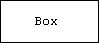
\includegraphics[width=2.589cm,height=1.138cm]{img/ref53.jpg} 

use the sequence

\begin{expara}

T1: {\textbackslash}L-{}-{}-{}-{}-{}-{}-{}-{}-R

T2: {\textbackslash}{\textbar} \ Box \ \ \ {\textbackslash}{\textbar}

T3: {\textbackslash}l-{}-{}-{}-{}-{}-{}-{}-{}-r

\end{expara}

This applies to all headers of screens in \PrBtq{} and \PrBtuser{}.

To display a ``\exampletext{{\textbackslash}}'' in a header it must be ``escaped'' with a preceding
``\exampletext{{\textbackslash}}'' like this ``\exampletext{{\textbackslash}{\textbackslash}}''.

\subsubsection{Changing message files}
A few tips may be useful:

\begin{itemize}
\item Tabs don't work in messages, since they may displayed anywhere on the screen; use multiple spaces instead.
\item Keep the messages reasonably short, this avoids having to redraw large areas of the screen just to display a message and obliterate
everything else going on.
\item When re-defining keys, don't forget to adjust the help and error messages to correspond, and make sure that they are all
consistently re-defined throughout all the states of all the programs.
\end{itemize}
Please note that there is nothing ``magic'' about the code numbers for global and local keystrokes. As distributed
the state codes 400 up to 499 are assigned to global keystrokes, and 500 upwards to local ones. If, for example, it would be required to
define a different help key in different places, then re-define \exampletext{1K400} etc.

Likewise, the order of access to screens in \PrBtq{} can be changed by redefining local versions of the quit key (405) and
selection of job and variable screens.

\subsection{Environment variables.}
The default set of directory and file names used by \ProductName{} is ``built in'', but most can be changed by
assignment to environment variables. The relevant environment variables have already been described in relevant sections. To recap they are:

\begin{center}
\begin{tabular}{|l l l|}
\hline
\bfseries Variable & \bfseries Default & \bfseries Description\\\hline
\filename{BTQCONF} & \filename{\$SPHELPDIR/btq.help} & \PrBtq{} message file\\ 
\filename{BTRESTCONF} & \filename{\$SPHELPDIR/btrest.help} & message file for other utilities\\
\filename{BTUSERCONF} & \filename{\$SPHELPDIR/btuser.help} & \PrBtuser{} message file\\
\filename{FILEMONCONF} & \filename{\$SPHELPDIR/filemon.help} & \PrBtfilemon{} message file\\ 
\filename{MAILER} & \filename{/bin/mail} & program used to send mail\\
\filename{SPHELPDIR} & \helpdir{} & message files\\
\filename{SPOOLDIR} & \spooldir{} & internal databases\\
\filename{SPROGDIR} & \progsdir & internal programs\\
\filename{XMBTQCONF} & \filename{\$SPHELPDIR/xmbtq.help} & \PrXmbtq{} message file\\
\filename{XMBTRCONF} & \filename{\$SPHELPDIR/xmbtr.help} & \PrXmbtr{} message file\\
\filename{XMBTUSERCONF} & \filename{\$SPHELPDIR/xmbtuser.help} & \PrXmbtuser{} message file\\\hline
\end{tabular}
\end{center}
These variables (excluding those starting with \exampletext{SP}) may be set individually by users, to get
their own help files, for instance.

Notice the use of environment variables in the default values. This allows the names of files to depend on the values of other environment
variables. It is useful to extend this approach to allow, for instance, customisation based on the terminal type by using the
\filename{\$TERM} environment variable.

\section{Variation of search order}
The order in which \configurationfile{} files are scanned, either to locate message files, or to read options, may be varied from the default if required.

A keyword, optionally placed in the Master configuration file \masterconfig, in each case may be used to vary this.

\subsection{Search order for message files}
The default search order, for example with \PrBtq{}, which searches for a file named in the variable \filename{BTQCONF}, is to look:

\begin{enumerate}
\item As specified in a \configurationfile{} file in the current directory.
\item As specified in the environment variable of that name. \item specified in a \homeconfigpath{} file off the user's home directory.
\item In a standard place, namely \filename{btq.help} in the system help files directory, by default \linebreak[4]\helpdir.
\end{enumerate}
This order may be respecified by assigning a ``PATH'' variable style value to the environment variable \helppathvar{}, consisting of
directory names separated by colons. The user's home directory may be denoted by ``\filename{\~{}}'' and any other
user's home directory by ``\exampletext{\~{}user}''. Any environment variables are fully expanded.

If a directory name is relative (not starting with ``\filename{/}''), it is taken as being relative to the directory from which the program was started.
The current directory should be represented as just ``\exampletext{.}''.

Finally the environment is represented as a ``\filename{!}''.

Thus the default search order is represented as:

\begin{expara}

\helppathvarname={\textquotedbl}.:!:\~{}:@{\textquotedbl}

\end{expara}

which causes the search to start in the current directory, then the
environment, then in the home directory, then in the new home directory configuration file \homeconfigpath.
Note that there is no way of suppressing the fallback to the standard location in the system help files directory.

It might be relevant for example, for a French user, with copies of the help files in a separate directory, to set a different search path,
thus:

\begin{expara}

\helppathvarname={\textquotedbl}.:!:/usr/spool/batchhelp/French{\textquotedbl}

\end{expara}

This will affect all \ProductName{} user-level programs, which search for a help file named by a keyword listed above. (It will also affect \OtherProductName{} programs, unless the environment assignment is made in \masterconfig{} only).

\subsection{Search order for program options}
An almost identical system is used for program options, with the keyword \configpathvar{} except that the search is in the
opposite order. Also the additional symbol ``-'' is used for command-line options.

The default is therefore:

\begin{expara}

\configpathvarname={\textquotedbl}@{}:!:.:-{\textquotedbl}

\end{expara}

Indicating the search first in the home directory, then the environment, then the current directory, and finally the command line options.

Note that it is possible to turn off the interpretation of command line options, if required, in this way, by omitting the
``\exampletext{{}-}'', limiting the command line arguments to, for example, just job numbers for \PrBtjchange{} etc.

Assignments to this will affect all \ProductName{} user-level programs (and also \OtherProductName{} user-level programs,
unless the assignment is made in \masterconfig only).

\subsection{Freezing options}
The \exampletext{+freeze-home} and \exampletext{+freeze-current} options in the user level commands and equivalent on-screen facilities
in \PrBtq{} and \PrXmbtq{} etc are not affected by these options, the software does not attempt to ``backwards-interpret'' these paths. In
particular please note that these facilities save all of the current values of these options regardless of whether they are default values
or where they were read from, so you may want to ``prune'' the values of the options saved.

